\documentclass[a4paper]{article}

\usepackage[utf8]{inputenc}
\usepackage[portuguese]{babel}
\usepackage{a4wide}
\usepackage[pdftex]{hyperref}
\usepackage{graphicx}
\usepackage{wrapfig}
\usepackage{amsmath}
\usepackage{caption}
\usepackage{subcaption}
\usepackage{tikz}
\usepackage{pgfplots}
\pgfplotsset{compat=1.10}
\usepgfplotslibrary{fillbetween}
\usepackage{pgfplots}
\usetikzlibrary{patterns}
\usepackage{float}



\begin{document}

\begin{titlepage}
\begin{center}



\includegraphics[width=0.4\textwidth]{logo}\\[0.3cm]

{\large Universidade do Minho - Escola de Engenharia}\\[0.5cm]

{\large Relatório do trabalho prático de Base de Dados}\\[0.5cm]



% Title
\rule{\linewidth}{0.5mm} \\[0.4cm]
{ \huge \bfseries Sistema de Gestão de Turnos Práticos \\[0.4cm] }
\rule{\linewidth}{0.5mm} \\[1.5cm]

% Author and supervisor
\noindent
\begin{minipage}{0.4\textwidth}
  \begin{flushleft} \large
    \emph{Autores :}\\
    Diana Costa \textsc{(A78985)}\\
    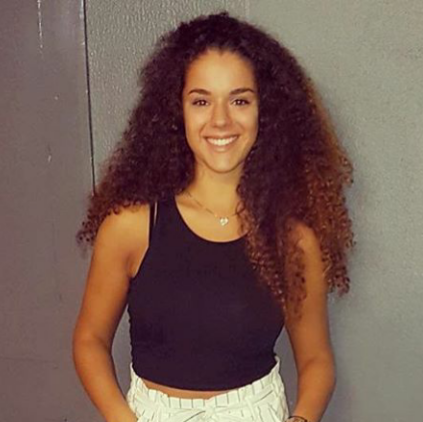
\includegraphics[width=1.5cm]{diana}\break
    Marcos Pereira \textsc{(A79116)}\\
    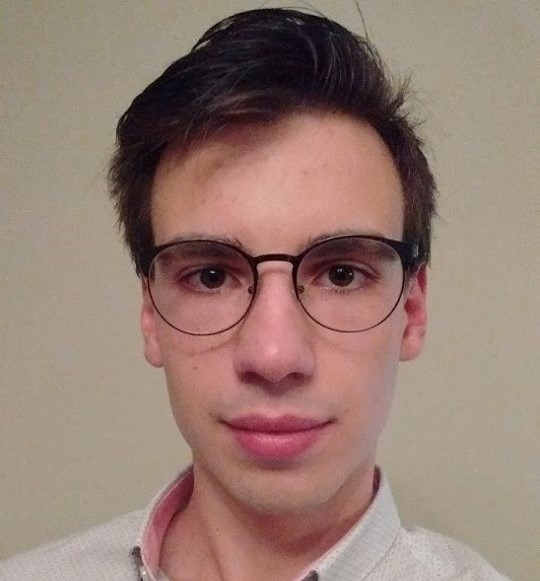
\includegraphics[width=1.5cm]{marcos}\break
    Sérgio Oliveira\textsc{(A77730)}\\
    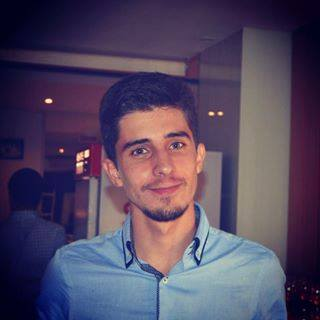
\includegraphics[width=1.5cm]{sergio}\break
    Vitor Castro\textsc{(A77870)}\\
    
\includegraphics[width=1.5cm]{vitor}\break
  \end{flushleft}
\end{minipage}%
\vfill

% Bottom of the page
{\large Versão 1.0 \\ \today}

\end{center}
\end{titlepage}


\begin{abstract}

\hspace{3mm}Neste relatório será feita

\end{abstract}

\pagebreak
\tableofcontents

\pagebreak

\section{Definição do Sistema}
\label{sec:1}

\subsection{Contexto de aplicação do sistema}
\subsection{Fundamentação da implementação da base de Dados}
\subsection{Análise da viabilidade do processo}

\section{Levantamento e Análise de Requisitos}
\label{sec:2}

\subsection{Método de levantamento e de análise de requisitos adotado}

\subsection{Requisitos levantados}
\subsubsection{Requisitos de descrição}
\subsubsection{Requisitos de exploração}
\subsubsection{Requisitos de controlo}

\subsection{Análise geral dos requisitos}

\section{Modelação Concetual}
\label{sec:3}

\subsection{Apresentação da abordagem de modelação realizada}
\subsection{Identificação e caracterização das entidades}
\subsection{Identificação e caracterização dos relacionamentos}
\subsection{Identificação e caracterização das Associação dos Atributos com as Entidades e Relacionamentos}
\subsection{Detalhe ou generalização de entidades}
\subsection{Apresentação e explicação do diagrama ER}
\subsection{Validação do modelo de dados com o utilizador}

\section{Modelação Lógica}
\label{sec:4}

\subsection{Construção e validação do modelo de dados lógico}
\subsection{Desenho do modelo lógico}
\subsection{Validação do modelo através da normalização}
\subsection{Validação do modelo com interrogações do utilizador}
\subsection{Validação do modelo com as transações estabelecidas}
\subsection{Reavaliação do modelo lógico (se necessário)}
\subsection{Revisão do modelo lógico com o utilizador}

\section{Implementação Física}
\label{sec:5}

\subsection{Seleção do sistema de gestão de bases de dados}
\subsection{Tradução do esquema lógico para o sistema de gestão de bases de dados escolhido em SQL}
\subsection{Tradução das interrogações do utilizador para SQL (alguns exemplos)}
\subsection{Tradução das transações estabelecidas para SQL (alguns exemplos)}
\subsection{Escolha, definição e caracterização de índices em SQL (alguns exemplos)}
\subsection{Estimativa do espaço em disco da base de dados e taxa de crescimento anual}
\subsection{Definição e caracterização das vistas de utilização em SQL (alguns exemplos)}
\subsection{Definição e caracterização dos mecanismos de segurança em SQL (alguns exemplos)}
\subsection{Revisão do sistema implementado com o utilizador}

\pagebreak

\section{Conclusões e Trabalho Futuro}
\label{sec:6}

\section{Referências Bibliográficas}
\label{sec:7}

FORMATO HARVARD


\end{document}
